\documentclass[report,gutter=10mm,fore-edge=10mm,uplatex,dvipdfmx]{jlreq}

\usepackage{lmodern}
\usepackage{amssymb,amsmath}
\usepackage{ifxetex,ifluatex}
\usepackage{actuarialsymbol}
\usepackage[]{natbib}
\RequirePackage{plautopatch}

% maru suji ① etc.
\usepackage{tikz}
\newcommand{\cir}[1]{\tikz[baseline]{%
\node[anchor=base, draw, circle, inner sep=0, minimum width=1.2em]{#1};}}

\usepackage{comment}

\begin{comment}

\ifnum0\ifxetex1\fi\ifluatex1\fi=0 % if pdftex
  \usepackage[T1]{fontenc}
  \usepackage[utf8]{inputenc}
  \usepackage{textcomp} % provide euro and other symbols
\else % if luatex or xetex
  \usepackage{unicode-math}
  \defaultfontfeatures{Scale=MatchLowercase}
  \defaultfontfeatures[\rmfamily]{Ligatures=TeX,Scale=1}
\fi
% Use upquote if available, for straight quotes in verbatim environments
\IfFileExists{upquote.sty}{\usepackage{upquote}}{}
\IfFileExists{microtype.sty}{% use microtype if available
  \usepackage[]{microtype}
  \UseMicrotypeSet[protrusion]{basicmath} % disable protrusion for tt fonts
}{}
\makeatletter
\@ifundefined{KOMAClassName}{% if non-KOMA class
  \IfFileExists{parskip.sty}{%
    \usepackage{parskip}
  }{% else
    \setlength{\parindent}{0pt}
    \setlength{\parskip}{6pt plus 2pt minus 1pt}}
}{% if KOMA class
  \KOMAoptions{parskip=half}}
\makeatother
\usepackage{xcolor}
\IfFileExists{xurl.sty}{\usepackage{xurl}}{} % add URL line breaks if available
\IfFileExists{bookmark.sty}{\usepackage{bookmark}}{\usepackage{hyperref}}
\hypersetup{
  hidelinks,
  pdfcreator={LaTeX via pandoc}}
\urlstyle{same} % disable monospaced font for URLs
\usepackage{longtable,booktabs}
% Correct order of tables after \paragraph or \subparagraph
\usepackage{etoolbox}
\makeatletter
\patchcmd\longtable{\par}{\if@noskipsec\mbox{}\fi\par}{}{}
\makeatother
% Allow footnotes in longtable head/foot
\IfFileExists{footnotehyper.sty}{\usepackage{footnotehyper}}{\usepackage{footnote}}

\end{comment}
%\makesavenoteenv{longtable}
\setlength{\emergencystretch}{3em} % prevent overfull lines
\providecommand{\tightlist}{%
  \setlength{\itemsep}{0pt}\setlength{\parskip}{0pt}}
\setcounter{secnumdepth}{-\maxdimen} % remove section numbering

\author{kazuyoshi}
\date{}

\newcommand{\problem}[1]{\subsubsection{#1}\setcounter{equation}{0}}
%\newcommand{\answer}[1]{\subsubsection{#1}}
\newcommand{\answer}[1]{\subsubsection{解答}}

%Pdf%\newcommand{\wakumaru}[1]{\framebox[3zw]{#1}}
\newcommand{\wakumaru}[1]{#1}






\begin{document}
\chapter{保険1 その他}
\section{1.   実務基準, 監督指針, 施行規則, 業法}

\subsection{実務基準}

\subsection{監督指針}

\subsection{施行規則}

\subsection{業法}

\problem{2022 生保2問題 1(1)【監督指針】}

「保険会社向けの総合的な監督指針」
【Ⅱ-2-1 責任準備金等の積立の適切性】について、以下
の(a)~(g)の空欄に当てはまる適切な語句または数値を記入しなさい。(7点)

\begin{itemize}
 \item [(ア)]「Ⅱ-2-1-2 積立方式(2)」においては以下が規定されている。\\
「第一分野及び第三分野において、保険会社の業務又は財産の状況及び保険契約の特性等
に照らし特別な事情がある場合に、保険数理に基づき、合理的かつ妥当なものとして、いわゆるチルメル式責任準備金の積立てを行っている場合には、 (a) に照らしチルメル歩合が妥当なものとなっているか。」
 \item [(イ)]「Ⅱ-2-1-2 積立方式(4)」においては以下が規定されている。\\
「特定の疾病による所定の状態、所定の身体障害の状態、所定の要介護状態その他の保険料
払込の免除事由に該当し、以後の保険料払込が免除されることとなった保険契約のうち、(b)の
可能な保険契約に係る責任準備金については、最終の保険期間満了日まで全て(b)が行われるものとして計算した金額を積み立てることとなっているか。」
\item[(ウ)]「Ⅱ-2-1-2 積立方式(5)」においては以下が規定されている。\\
「 (c) Ⅰ及びⅣにおける「 (d) 」に係る積立基準並びに積立限度の設定につい
ては、手術給付、介護給付その他の保険給付のリスクに応じたものとなっているか。
」
\item[(エ)]「Ⅱ-2-1-2 積立方式(7)④」においては以下が規定されている。\\
「ストレステスト及び (e) の基礎率を同じくする契約区分は同一のものを使用するこ
ととする。」
\item[(オ)]「Ⅱ-2-1-3-1 保険料積立金の積立(1)標準的方式①」においては以下が規定さ
れている。\\
「通常予測されるリスクに対応するものとして、標準的な計算式(
「一般勘定における最低
保証に係る保険金等の支出現価」から「一般勘定における最低保証に係る純保険料の収入現
価」を控除する形式の計算式)によって、概ね (f) %の事象をカバーできる水準に対
応する額を算出するものとなっているか。」
\item[(カ)]「Ⅱ-2-1-3-1 保険料積立金の積立(2)代替的方式④」において、平成8年2月
29日大蔵省告示第48号に列記する国内株式等の期待収益率及び (g) について、当
該告示に定めるものを使用する場合を除き、過去の実績や将来の資産運用環境の見通し、リ
スク中立の観点等から、合理的かつ客観的根拠に基づき定められる必要があることが規定
されている。
\end{itemize}
\answer{}
\begin{itemize}
\item[ (a): ] 新契約費水準
\item[ (b): ] 自動更新
\item[ (c): ] 危険準備金
\item[ (d): ] その他のリスク
\item[ (e): ] 負債十分性テスト
\item[ (f): ] 50
\item[ (g): ] ボラティリティ
\end{itemize}

\problem{2022 生保2問題 1(2)【業法】}
生命保険会社の保険計理人の職務(保険業法第121条)について、以下の(a)~(e)の空
欄に当てはまる適切な語句を記入しなさい。
(5点)

\begin{itemize}
\item[(ア)] 保険計理人は、毎決算期において、次に掲げる事項について、内閣府令で定めるところにより確認し、その結果を記載した(a)を(b)に提出しなければならない。
\begin{itemize}
\item[・]  内閣府令で定める保険契約に係る責任準備金が (c) に基づいて積み立てられているかどうか。
\item[・]  契約者配当又は社員に対する剰余金の分配が(d)に行われているかどうか。
\item[・]  その他内閣府令で定める事項
\end{itemize}
\item[(イ)] 保険計理人は、(ア)の(a)を(b)に提出した後、遅滞なく、その写しを(e)に提出しなければならない。
\item[(ウ)] (e)は、保険計理人に対し、(イ)の(a)の写しについてその説明を求め、その他その職務に属する事項について意見を求めることができる。
\item[(エ)] 上記に定めるもののほか、(ア)の(a)に関し必要な事項は、内閣府令で定める。
\end{itemize}

\answer{}
\begin{itemize}
\item[ (a): ] 意見書
\item[ (b): ] 取締役会
\item[ (c): ] 健全な保険数理
\item[ (d): ] 公正かつ衡平
\item[ (e): ] 内閣総理大臣
\end{itemize}
※(e)は「金融庁(長官)」も正答とした。

\problem{2022 生保2問題 1(4)【監督指針】}
「保険会社向けの総合的な監督指針」
【Ⅱ-2-4 生命保険会社の区分経理の明確化】について、
以下の(a)~(e)の空欄に当てはまる適切な語句を記入しなさい。
(5点)

Ⅱ-2-4-2 主な着眼点

各生命保険会社においては、適切な区分経理を行うため、例えば、以下のような考えに基づく
区分経理に関する管理方針を策定しているか。また、区分経理の状況が、取締役会その他これ
に準ずる機関に対して報告されているか。

(1)〜(6) (省略)

(7)各区分間の取引等
\begin{itemize}
\item[①] 資産区分間の取引\\
資金移動(流入・流出)管理、 (a) 確保、ポートフォリオの改善等、必要な取引とし、市場価格等の適正な価格をもって適切に管理する。
\item[②]商品区分と全社区分との取引\\
\begin{itemize}
\item[ア.] 現預金等の貸借
\begin{itemize}
\item[(ア)] 商品区分又は全社区分毎に区別して管理する。
\item[(イ)] (b)が継続しないよう限度額等を設ける。
\end{itemize}
\item[イ.] 現預金等以外の貸借
\begin{itemize}
\item[(ア)]  (c) から (d) への貸付は、異常な保険金の支払い、新商品の販売に伴う事業運営資金、その他やむを得ない事情がある場合に限る。
\item[(イ)]  (d) から (c) への貸付は、 (c) の規模が小さいために、その機能を十分に果たすことができない場合に限る。
\item[(ウ)] 上記の貸借は、金額、利率(貸付期間に応じた市中金利等を基に設定すること)、期限その他の返済条件をあらかじめ定める。
\item[(エ)] 貸付条件の緩和や債務免除は、回収が不可能な損失が発生している場合等、やむを得ない事情がある場合を除き、 (e) 。なお、貸付条件の緩和等を行った後に利益が生じた場合は、当該利益を返済に充てるものとする。
\end{itemize}
\item[ウ.] 出資 (省略)
\item[エ.] その他の取引 (省略)
\end{itemize}
\end{itemize}

\answer{}
\begin{itemize}
\item[ (a): ]  流動性
\item[ (b): ]  借越し
\item[ (c): ]  全社区分
\item[ (d): ]  商品区分
\item[ (e): ]  行わない
\end{itemize}

\problem{2022 生保1問題 1(1)【施行規則】}
保険業法施行規則第 10 条について、次の①~⑤に適切な語句を記入しなさい。(5点)

第 10 条(\wakumaru{①}の記載事項)

免許申請者は、法第3条第4項の生命保険業免許の申請の場合にあっては第1号から第6号まで及び第8号に掲げる事項を、
(略)法第4条第2項第4号に掲げる書類に記載しなければならない。

\begin{itemize}
\item[ 一  ] 保険料の計算の方法(略)に関する事項
\item[ 二  ] 責任準備金(法第\wakumaru{②}条第1項の責任準備金をいう。(略))の計算の方法(略)に関する事項
\item[ 三  ] 返戻金の額その他の被保険者のために積み立てるべき額を基礎として計算した金額(以下「\wakumaru{③}」という。)の計算の方法及びその基礎に関する事項
\item[ 四  ] 第 30 条の5第1項第1号の社員配当準備金又は第 64 条第1項の契約者配当準備金及び社員に対する剰余金の分配又は契約者配当の計算の方法に関する事項
\item[ 五  ] \wakumaru{④}の計上に関する事項
\item[ 六  ] 保険金額、保険の種類又は\wakumaru{⑤}を変更する場合における計算の方法に関する事項
\item[ 七  ]( 略)
\item[ 八  ] その他保険数理に関して必要な事項
\end{itemize}

\answer{}
\begin{itemize}
\item[ ① ] 保険料及び責任準備金の算出方法書 
\item[ ② ] 116 
\item[ ③ ] 契約者価額 
\item[ ④ ] 未収保険料
\item[ ⑤ ] 保険期間
\end{itemize}
\answer{}

\problem{2021 生保1問題1(1)【実務基準】}
アセット・シェアについての生命保険会社の保険計理人の実務基準(以下、
「実務基準」とし、解説書を含む)に関する次の①~⑤について、下線
場合は×を記入するとともに、下線部分が正しい場合は○を記入し、誤っている
部分を正しい表現に改めなさい。

\begin{itemize}
 \item [①] 実務基準第 23 条(アセット・シェアと代表契約の選定)において、アセット・シェア方式とは、「代
表契約の設定などにより、会社の資産の\underline{簿価}に対する保険契約の貢献度を評価する手法」を指す。
 \item [②] 実務基準第 23 条(アセット・シェアと代表契約の選定)において、アセット・シェアに基づく配当
確認のために設定した選定単位の代表契約は、実際に当該選定単位に存在する契約である必要\underline{がある}。
\item[③] 実務基準第 24 条(当年度末アセット・シェアの確認)において、当年度末アセット・シェアは、以下の考え方に基づいて計算することとなっている。\\
当年度末アセット・シェア = 前年度末アセット・シェア + 保険料 + 資産運用収益\\
±評価差額金(税効果控除前)増減額 - 支払保険金など - \underline{予定事業費} - 税金\\
- 支払配当金 ± 法人税等調整額 ± 全社区分調整額
\item[④] 実務基準第 24 条(当年度末アセット・シェアの確認)において、選定した代表契約のアセット・シ
ェアの初期値は、合理的かつ適正に決定しなければならないとされている。このとき、アセット・
シェアの初期値が負値となることは\underline{認められる}。
\item[⑤] 実務基準第 25 条(将来のアセット・シェアの確認)において、代表契約の将来のアセット・シェア
は、金利、株価、保険事故発生率、経費上昇率などのパラメータが、
「直近の実績」のまま将来も継
続することとして、計算しなければならないとされている。このとき、保険事故発生率の「直近の
実績」は、阪神・淡路大震災のような巨大リスクによる保険事故発生分を除外した保険事故発生率
とすること\underline{ができる}。
\end{itemize}
\answer{}
\begin{itemize}
\item[ ① : ]  ×:時価 
\item[ ② : ]  ×:はない 
\item[ ③ : ]  ×:事業費 
\item[ ④ : ]  ○ 
\item[ ⑤ : ]  ○
\end{itemize}

\problem{2021 生保1問題1(3)【監督指針】}

保険会社向けの総合的な監督指針「Ⅳ-5-3 契約者価額」(令和3年8月改正)について、次の①~⑤に適切な語句を記入しなさい。

Ⅳ-5-3 契約者価額

(1)解約返戻金については、支出した事業費及び①の損失、保険設計上の仕組み等に照らし、合理的かつ妥当に設定し、保険契約者にとって不当に不利益なものとなっていないか。

(2)②を利用した商品について、解約返戻金額の計算基礎を設定する時期と解約時期の間に生じる③や、解約に伴う運用資産の売却に係る④等に備えるために係数を定める場合、その係数については、⑤の高度化や解約に伴って見込まれる④との整合性等に照らして、合理的かつ妥当な水準に設定し、保険契約者にとって不当に不利益なものとなっていないか。

\answer{}
\begin{itemize}
\item[ ① : ] 投資上 
\item[ ② : ] MVA 
\item[ ③ : ] 金利変動
\item[ ④ : ] 取引費用 
\item[ ⑤ : ] リスク管理
\end{itemize}

\problem{2020 生保1問題1(1)【監督指針】}
保険会社向けの総合的な監督指針「Ⅳ-6 審査手続」について、次のA~Eに適切な語句を記入しなさい。

Ⅳ-6-1 保険商品の認可・届出に係る審査期間の取扱い

保険商品の認可・届出に係る審査期間は、認可については規則第 246 条第1項第 12 号に規定する標準処理期間として
\wakumaru{A}日、また、届出については法第 125 条第1項により\wakumaru{A}日とされているところであるが、商品開発の迅速化に資するという観点から、審査期間の短縮に努めるものとする。(中略)

Ⅳ-6-2 保険商品審査にあたっての手順

審査にあたっては、届出又は認可申請に際し保険会社が概要書(様式・参考資料編その他報告等様式集 Ⅳ-6-2 別紙1~3)に所定の内容を記載したうえでこれを添付している場合には、概要書を用いて迅速かつ効率的な審査を行うこととする。(以下略)

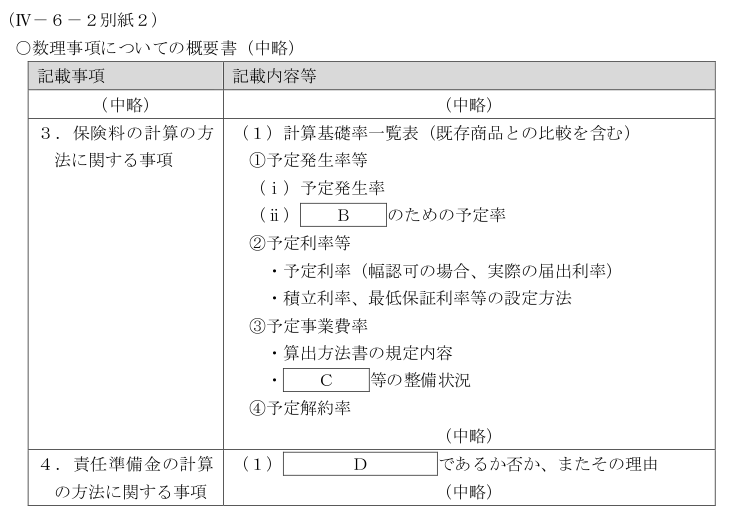
\includegraphics[scale=0.5]{./images/Prob2020-1-1-1-1.png}\\
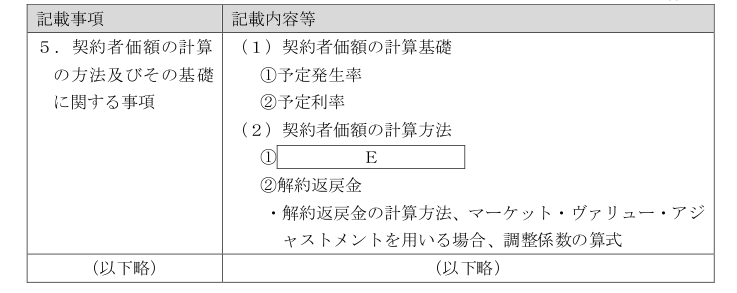
\includegraphics[scale=0.5]{./images/Prob2020-1-1-1-2.png}

\answer{}

\begin{itemize}
\item[ A:]  90 
\item[ B:]  保険料免除 
\item[ C:]  社内規定 
\item[ D:]  標準責任準備金対象契約 
\item[ E:]  保険契約上の責任準備金
\end{itemize}


\problem{2020 生保1問題1(2)}
アセット・シェアの配当率設定・確認への活用について、次の①、②の各問に答えなさい。\vspace{1zh}

\noindent ① 「生命保険会社の保険計理人の実務基準」第 23 条第4項に定める、代表契約の選定単位を設定す
る際に最低限区分しなければならない項目を3つ挙げなさい。(3点)\\
② 「生命保険会社の保険計理人の実務基準」第 23 条第5項に定める、①の他にさらに細かく区分す
ることができる項目を4つ挙げなさい。(2点)
\answer{}
① 区分経理の商品区分、保険事故の種類、契約経過年度

② 基礎書類上の保険種類、販売経路、危険選択手法、性別、契約年齢、保険料払込方法、保険金
額、保険期間 (これらのうちから4つを解答すること。)

\problem{2019 生保1問題 1(2)【監督指針】}
保険会社向けの総合的な監督指針「Ⅱ-2-5 商品開発に係る内部管理態勢」について、次の①~⑤に適切な語句を記入しなさい。

\noindent{}Ⅱ-2-5 商品開発に係る内部管理態勢\\
Ⅱ-2-5-1 意義

保険商品の内容は「普通保険約款」及び「\wakumaru{①}」に、料率については「\wakumaru{②}」に記載されてお
り、新商品の開発、商品内容の変更は、これらの変更を通じて行われている。

保険会社より商品の\wakumaru{③}申請が行われた場合、監督当局としては、契約内容が保険契約者等の
保護に欠けるおそれがないか、不当な差別的取扱いをするものではないか、契約内容が公序良俗を害
するものではないか等の保険業法に定める基準に適合するものであるか審査を行い、適当と認めら
れたものについて、これを\wakumaru{③}することとしている。

近年、保険商品には、わが国における社会の構造的変化・経済活動の多様化等に伴い、国民の生活
保障ニーズの高まり、新たなリスクの発生など、保険契約者ニーズに対応すべく多様化が求められて
いる。

こうしたニーズに応え、保険会社が商品開発を行うにあたっては、保険業法等の法令等を踏まえ、
\wakumaru{④}に基づき、リスク面、財務面、\wakumaru{⑤}、法制面等あらゆる観点から検討する内部管理態勢の整備が求められているところである。

\answer{}
\begin{itemize}
\item[ ① :] 事業方法書
\item[ ② :] 保険料及び責任準備金の算出方法書
\item[ ③ :] 認可
\item[ ④ :] 自己責任原則
\item[ ⑤ :] 募集面
\end{itemize}

\problem{2018 生保1問題 1(4)【監督指針】}

保険会社向けの総合的な監督指針「Ⅱ-2-5 商品開発に係る内部管理態勢」
「Ⅳ.保険商品審査上の留意点等」について、次のA〜Gに適切な語句を記入しなさい。

Ⅱ-2-5 商品開発に係る内部管理態勢

【省略】

Ⅱ-2-5-2 主な着眼点

(1)~(4)【省略】

(5)関連部門との連携

① ~ ②【省略】

③ 商品内容の概略決定にあたり、\wakumaru{A}、保険引受リスク、コンプライアンス、販売計画、システム開発、保険商品特有の道徳的危険等についての課題及び検討内容等を各関連部門において議論しているか。

なお、\wakumaru{A}については、商品ごとに保険会社の経営実態を踏まえた実現可能性の高い保険事故発生率並びに事業費その他のシナリオに基づき問題ないものとなっていることを確認しているか。

④ 社内規定等に定める付加保険料の算出方法が\wakumaru{B}かつ妥当なものであり、かつ、その算出された付加保険料が不当に差別的なものとなっていないことが確保されているか。特に、付加保険料の割増引きを設定する場合には、契約方法、保険料の払込方法等に基づいたものとなっており、事実上の\wakumaru{C}(法第 300 条第1項第5号)になっていないことに留意する。
【省略】

Ⅳ.保険商品審査上の留意点等

【省略】

Ⅳ-1 共通事項

第一分野、第二分野、第三分野の商品審査に係る共通事項として、特に以下の点に留意して審査することとする。

Ⅳ-1-1 普通保険約款及び特約の記載事項について

普通保険約款及び特約の記載事項については、\wakumaru{D}等の保護の観点から、明確かつ平易で、簡素なものとなっているかに留意することとする。

Ⅳ-1-2 保障又は補償の内容

\begin{itemize}
\item[ (1) ] 保障又は補償(以下、「保障等」という。)の内容が法第3条第4項から第6項に適合しているか。
\item[ (2) ] 保障等の内容が\wakumaru{D}等の\wakumaru{E}及び利便に適合しているか。
\item[ (3) ] 適正な死亡率や発生率が組み込まれているか、補償の内容が偶然性及び損害のてん補性を有しているかなど、\wakumaru{F}の有無に係る検討が十分行われているか。
\item[ (4) ] 支払事由に比して極端に高額な保険金が支払われるものや免責事由が極端に少ないもの、あるいは実損額を上回る保険金が支払われるものなどについては、射倖性が高いものとなっていたり、\wakumaru{G}が生じやすいものとなっていないか、検討が十分に行われているか。
\item[ (5) ] 支払事由が明確なものとなっているか。
\end{itemize}
【以下省略】
\answer{}
\begin{itemize}
\item[ A: ] 収支予測
\item[ B: ] 合理的
\item[ C: ] 特別利益の提供
\item[ D: ] 保険契約者
\item[ E: ] 需要
\item[ F: ] 保険性
\item[ G: ] モラルハザード
\end{itemize}

\problem{H29 生保1問題 1(1)【監督指針】}
保険会社向けの総合的な監督指針における団体保険又は団体契約の保険商品審査上の留意点につい
て、次の A~E に適切な語句を記入しなさい。

Ⅳ-1-14 団体保険又は団体契約の取扱い

団体保険又は団体契約については、以下の点に留意して審査することとする。

(1)団体及び被保険団体の範囲が、明確に定められているか。

(2)商品特性、募集管理態勢及び契約管理態勢、 A やリスク管理の状況等に照らし、 B
の排除や保険収支の安定等を目的として団体要件(例えば、一契約の最低被保険者数、 C
、最低加入率等)を定める必要がある場合、適切な団体要件を定めているか。
また、その場合に、被保険団体の区分(全員加入団体、任意加入団体)及び団体の区分に応じて、明確に定められているか。

(3)職域を基礎とする団体保険又は団体契約において、退職者及び退職者の配偶者等(以下、本項において「退職者等」という。)を引き続き被保険団体に含める場合は、以下の点を満たしているか。

① 団体が、退職者等に係る異動状況の把握及び保険料の収納管理を適切に行うための事務処理能力を有していること。
② 退職者等を被保険団体に含めること及び、これに伴って将来的に想定される退職者等の占める割合が
Dすることによる影響を踏まえ、A リスクに見合った保険料又は E 等の設定となっていること。

\answer{}
\begin{itemize}
\item[ A.] 保険引受 
\item[ B.] モラルリスク 
\item[ C.] 最高保険金額倍数 
\item[ D.] 上昇
\item[ E.] 配当方式
\end{itemize}

\problem{H29 生保1問題 1(3)【業法,実務基準】}
配当(剰余金の分配・契約者配当)の設定・確認におけるアセット・シェアの活用について、次の①
~⑤に適切な語句を記入しなさい。

相互会社における剰余金の分配については、保険業法第 55 条の 2 において、剰余金の分配は公正か
つ\wakumaru{①}に行わなければならないことが規定されている。
これを受けて、保険業法施行規則第 30 条の2 において、
「相互会社が社員に対する剰余金の分配をする場合には、保険契約の特牲に応じて設定し
た区分ごとに、剰余金の分配の対象となる金額を計算」することとされている。すなわち、 
\wakumaru{②}を行ったうえでアセット・シェア方式や利源別方式等の方法で
剰余金の分配を行うことが示唆されている。

株式会社における契約者配当についても、保険業法第 114 条および保険業法施行規則第 62 条におい
て、同様に規定されている。

配当が公正・ \wakumaru{①}であることの確認においては、
代表契約の当年度末アセット・シェアの計算が必要となる。当年度末アセット・シェアの計算については、
「生命保険会社の保険計理人の実務基準」第24 条第 2 項において、以下のとおり定められている。\\ 
\vspace{1zh}
第 24 条(当年度末アセット・シェアの確認)\\
2.代表契約の当年度末アセット・シェアは、以下の考え方に基づいて計算する。

\begin{tabular}{ccl}
当年度末アセット・シェア&=&\wakumaru{③}+\wakumaru{④}+資産運用収益\\
 & ±&評価差額金(税効果控除前)増減額-支払保険金など \\
 &- &\wakumaru{⑤}-税金-支払配当金±法人税等調整額±全社区分調整額 \\
\end{tabular}
\answer{}
\begin{itemize}
 \item[①: ]衡平
\item[②: ]区分経理
\item[③: ]前年度末アセット・シェア 
\item[④: ]保険料 
\item[⑤: ]事業費
\end{itemize}

\problem{H28 生保1問題 1(1)【業法,施行規則】}
以下の保険業法および保険業法施行規則の抜粋について、次の①~⑤に適切な語句を記入しなさい。

【保険業法第3条(免許)】\\
【省略】

4.生命保険業免許は、第1号に掲げる保険の引受けを行い、又はこれに併せて第2号若しくは第3号に掲げる保険の引受けを行う事業に係る免許とする。
\begin{itemize}
\item[ 一 ] 人の\wakumaru{①}(当該人の …【中略】… 同じ。)に関し、一定額の保険金を支払うことを約し、保険料を収受する保険(次項ハに …【中略】… を除く。)
\item[ 二 ] 次に掲げる事由に関し、一定額の保険金を支払うこと又はこれらによって生ずることのある当該人の損害をてん補することを約し、保険料を収受する保険
\begin{itemize}
\item[ イ ] 人が\wakumaru{②}にかかったこと。
\item[ ロ ] \wakumaru{③}を受けたこと又は\wakumaru{②}にかかったことを原因とする人の状態
\item[ ハ ] \wakumaru{③}を受けたことを直接の原因とする人の死亡
\item[ ニ ] イ又はロに掲げるものに類するものとして内閣府令で定めるもの(人の死亡を除く。)
\item[ ホ ] イ、ロ又はニに掲げるものに関し、治療(治療に類する …【中略】… を含む。)を受けたこと。
\end{itemize}
\item[ 三 ] 次項第1号に掲げる保険のうち、再保険であって、前2号に掲げる保険に係るもの
 【省略】
\end{itemize}

【保険業法施行規則第4条(\wakumaru{②}等に類する事由)】

法第3条第4項第2号二に規定する内閣府令で定める事由は、次に掲げる事由とする。

\begin{itemize}
\item[ 一 ]  \wakumaru{④}及びこれを原因とする人の状態
\item[ 二 ]  \wakumaru{⑤}を要する身体の状態
\item[ 三 ]  老衰を直接の原因とする常時の介護を要する身体の状態
\item[ 四 ]  骨髄の提供及びこれを原因とする人の状態
\end{itemize}

\answer{}
\begin{itemize}
\item[ ①: ]  生存又は死亡
\item[ ②: ]  疾病
\item[ ③: ]  傷害
\item[ ④: ]  出産
\item[ ⑤: ]  不妊治療
\end{itemize}

\problem{H28 生保1問題 1(2)【大蔵省告示】}
大蔵省告示第233号(平成10年6月8日)について、次の①~⑤に適切な語句を記入しなさい。

第1条(財務再保険)

保険業法施行規則(以下「規則」という。)第71条第2項に規定する金融庁長官が定める再
保険は、保険会社が保険契約を再保険に付した場合において、当該再保険に付した部分に係る
\wakumaru{①}を移転することを約し、当該再保険に付した部分に係る保険契約から当該再保険に付
した後に発生することが見込まれる収益(以下 …【中略】… という。)を
\wakumaru{②}(受再 …【中略】… 同じ。)としてあらかじめ収受する再保険であって、次に掲げるすべての要件に該
当するものをいう。

一 【省略】
二 元受保険会社が受再保険会社から収受する\wakumaru{②}は\wakumaru{③}によるものであること。
三 【省略】
四 受再保険会社による\wakumaru{④}は、元受保険会社の再保険料の不払いによる場合を除き、できないものであること。
【省略】

第2条(種類)\\
【第1項省略】

2.前項第1号に掲げる\wakumaru{⑤}とは、受再保険会社が、元受保険契約(元受保険会社 …【中略】… 同じ。)に係るリスクのうち、当該再保険に付された部分に係る\wakumaru{①}を出再割合(受再保険会社 …【中略】… 同じ。)に応じて引き受け、当該引き受けた部分に係る責任準備金(保険業法 …【中略】… 同じ。)の積立て及び当該責任準備金に相当する額の資産の管理を行うものをいう。
【以下省略】

\answer{}
\begin{itemize}
\item[ ①: ]  すべてのリスク
\item[ ②: ]  出再保険受入手数料
\item[ ③: ]  現金
\item[ ④: ]  一方的な解約
\item[ ⑤: ]  共同保険式再保険
\end{itemize}


\problem{H27 生保1問題 1(1)【監督指針】}
保険会社向けの総合的な監督指針「Ⅳ-5 保険数理」について、次の①~⑦に適切な語句を記入しなさい。

\noindent{} Ⅳ-5 保険数理

算出方法書の審査にあたっては、特に以下の点に留意することとする。
\begin{itemize}
 \item [] Ⅳ-5-1 保険料\\
【省略】
 \item [] Ⅳ-5-2 責任準備金
\begin{enumerate}[(1)]
\item  (省略)
\item 商品の設計上、契約期間初期の給付を大きくすること若しくは将来の給付を減少させること又は
 保険料を後払いにすることについては、責任準備金が \wakumaru{①} とならないように設定されているか。
 なお、責任準備金の計算上、 \wakumaru{①} となる契約に係る責任準備金を \wakumaru{②} とする対応をとる場合
 においては、 \wakumaru{③} 確保に関する十分な検討がなされているかに留意する。
\item マーケット・ヴァリュー・アジャストメントの仕組みを持つ商品の責任準備金については、
\wakumaru{④} と \wakumaru{⑤} とのいずれか大きい額を積み立てることとなっているか。
\end{enumerate} 
\item [] Ⅳ-5-3 契約者価額\\
解約返戻金については、支出した\wakumaru{⑥}及び\wakumaru{⑦}の損失、保険設計上の仕組み等に照らし、合
理的かつ妥当に設定し、保険契約者にとって不当に不利益なものとなっていないか。
【以下省略】
\end{itemize}

\answer{}
\begin{itemize}
\item[ ①:]  負値
\item[ ②:]  ゼロ
\item[ ③:]  財務の健全性
\item[ ④:]  保険料積立金
\item[ ⑤:]  解約返戻金
\item[ ⑥:]  事業費
\item[ ⑦:]  投資上
\end{itemize}

\problem{H27 生保1問題 1(2)【実務基準】}
「生命保険会社の保険計理人の実務基準」第 23 条(アセットシェアと代表契約の選定)について、
次の A~E に適切な語句を記入しなさい。


\begin{enumerate}
 \item 保険計理人は、\wakumaru{A}として\wakumaru{B}を支払う契約については、代表契約を選定し、第 24 条および第 25 条の規定に従い、アセット・シェアに基づき配当を確認しなければならない。
 \item 
アセット・シェア方式とは、
「代表契約の設定などにより、会社の資産の時価に対する保険契約の
貢献度(アセット・シェア)を評価する手法」 であり、これにより求められた契約のアセット・
シェアと対応責任準備金との差額をネット・アセット・シェアという。
 \item 
保険計理人は、第 1 項の代表契約の選定に際しては、選定単位を設定し、各単位の当年度末有効契
約の収支状況を代表していると考えられる契約を、各選定単位の代表契約としなければならない。
 \item 
前項の選定単位は、以下の項目によって最低限区分して、設定しなければならない。
\begin{itemize}
 \item [①] \wakumaru{C}
 \item [②] 保険事故の種類
 \item [③] 契約経過年度
\end{itemize}
 \item 
第 3 項の選定単位は、前項の項目の他に、以下の項目によってさらに細かく区分することもできる。
\begin{itemize}
 \item [①]  基礎書類上の保険種類
 \item [②] \wakumaru{D}
\item [③] \wakumaru{E}
\item [④]  性別
\item [⑤]  契約年齢
\item [⑥]  保険料払込方法
\item [⑦]  保険金額
\item [⑧]  保険期間
\end{itemize}
\end{enumerate}
\answer{}

\begin{itemize}
\item [A: ] 最終精算
\item [B: ] 消滅時配当
\item [C: ] 区分経理の商品区分
\item [D: ] 販売経路
\item [E: ] 危険選択手法
\end{itemize}

\problem{H26 生保1問題 1(1)【施行規則】}
保険業法施行規則において生命保険会社が「保険料及び責任準備金の算出方法書」 に記載しなけれ
ばならないとされる事項について、次の①~⑤の空欄に当てはまる適切な語句を記入しなさい。

\begin{itemize}
\item[ ] 保険料の計算の方法に関する事項
\item[ ] 責任準備金の計算の方法に関する事項
\item[ ] \wakumaru{①}の額その他の被保険者のために積み立てるべき額を基礎として計算した金額の計算の方法及びその基礎に関する事項
\item[ ] 社員配当準備金又は\wakumaru{②}準備金及び社員に対する剰余金の分配又は\wakumaru{②}の計算の方法に関する事項
\item[ ] \wakumaru{③}の計上に関する事項
\item[ ] 保険金額、保険の種類又は\wakumaru{④}を変更する場合における計算の方法に関する事項
\item[ ] その他\wakumaru{⑤}に関して必要な事項
\end{itemize}

\answer{}
\begin{itemize}
\item[①:]  返戻金
\item[②:]  契約者配当
\item[③:]  未収保険料
\item[④:]  保険期間
\item[⑤:]  保険数理
\end{itemize}

\problem{H25 生保1問題 1(3)【施工規則】}
保険業法施行規則第71条および大蔵省告示第233号(平成10年6月8日)によって定義され
ている財務再保険について以下の①~③の空欄に当てはまる適切な語句を答え、下の表の各欄に
A~Cを埋めなさい。

\begin{tabular}{|l|c|c|c|}
 \hline
\multirow{2}{*}{}& \multicolumn{2}{c|}{将来収益に基づいた手数料を元受会社が受けるもの}
 &\multirow{2}{*}{その他}\\  \cline{2-3}
&告示第233号第1号の要件をすべて満たすもの&その他&\\ \hline
共同保険式  & & & \\ \hline
修正共同保険式 & & & \\ \hline
その他 & & & \\ \hline
\end{tabular}

\begin{itemize}
\item[ A:] 日本の法令上、「財務再保険」と定義されることにより、 \wakumaru{①}を\wakumaru{②}することができる。
\item[ B:] 日本の法令上、「財務再保険」と定義されないことにより、 \wakumaru{①}を\wakumaru{②}できず、 \wakumaru{③}として計上しなければならない。
\item[ C:] 日本の法令上、何の規制もない。
\end{itemize}
\answer{}

\begin{itemize}
\item[ ①: ] 手数料収入
\item[ ②: ] 収益認識
\item[ ③: ] 預かり金
\end{itemize}

\begin{tabular}{|l|c|c|c|}
 \hline
\multirow{2}{*}{}& \multicolumn{2}{c|}{将来収益に基づいた手数料を元受会社が受けるもの}
 &\multirow{2}{*}{その他}\\  \cline{2-3}
&告示第233号第1号の要件をすべて満たすもの&その他&\\ \hline
共同保険式  & A&B &C \\ \hline
修正共同保険式 &A &B & C \\ \hline
その他 & B & B & C\\ \hline
\end{tabular}

\problem{H24 生保1問題 1(3)【保険法】}
保険法に規定されている保険契約について、次の①~⑥の空欄に当てはまる適切な語句を答えなさい。

\begin{itemize}
\item[ ・ ] 生命保険契約とは、保険契約のうち、保険者が人の①又は②に関し一定の③を行うことを約するもの(傷害疾病定額保険契約に該当するものを除く。)をいう。
\item[ ・ ] 損害保険契約とは、保険契約のうち、保険者が一定の④によって生ずることのある損害を⑤することを約するものをいう。
\item[ ・ ] 傷害疾病定額保険契約とは、保険契約のうち、保険者が人の傷害疾病に基づき一定の③を行うことを約するものをいう。
\item[ ・ ] 傷害疾病損害保険契約とは、⑥のうち、保険者が人の傷害疾病によって生ずることのある損害(当該傷害疾病が生じた者が受けるものに限る。)を⑤することを約するものをいう。
\end{itemize}

\answer{}
\begin{itemize}
\item[ ① ]  生存
\item[ ② ]  死亡
\item[ ③ ]  保険給付
\item[ ④ ]  偶然の事故
\item[ ⑤ ]  てん補
\item[ ⑥ ]  損害保険契約
\end{itemize}



\problem{H22 生保1問題 1(2)【監督指針】}
「保険会社向けの総合的な監督指針」に規定されている団体保険又は団体契約の商品審査上の留意
点について、以下の①~⑤の空欄に当てはまる適切な語句を答えなさい。

\begin{itemize}
\item[] 団体及び被保険団体の範囲が、明確に定められていること。
\item[] 被保険団体の区分(全員加入団体、任意加入団体)及び団体の区分(第Ⅰ種から第Ⅳ種等)に応じて、例えば一契約の\wakumaru{①}及び\wakumaru{②}が明確に定められていること。
\item[] 職域を基礎とする団体保険又は団体契約において、\wakumaru{③}及び\wakumaru{③}の配偶者等を引き続き被保険団体に含める場合、異動状況の把握及び保険料の収納管理を適切に行うための事務処理能力を有していること。
\item[]  \wakumaru{③}等を被保険団体に含めること及び、これに伴って将来的に想定される\wakumaru{③}等の占める割合が上昇することによる影響を踏まえ、保険引受リスクに見合った\wakumaru{④}又は\wakumaru{⑤}等の設定となっていること。
\end{itemize}

\answer{}
\begin{itemize}
\item[ ①: ] 最低被保険者数
\item[ ②: ] 最高保険金額倍数
\item[ ③: ] 退職者
\item[ ④: ] 保険料
\item[ ⑤: ] 配当方式
\end{itemize}

\problem{H21 生保1問題 1(1)【大蔵省告示】}
次の再保険に関する説明文について、以下の①~⑦の空欄に適切な語句を解答用紙の所定の欄に記
入しなさい。

\begin{itemize}
\item[] 平成 10 年 大蔵省告示第 233 号においては、再保険契約のうち、元受会社が出再部分についてす
 べてのリスクを移転し、出再部分からの将来収益を出再保険受入手数料として収受するもので、か
 つ同告示第 1 条ならびに第 2 条の条件を同時に満たすものを\wakumaru{①}として定義している。
 この場合、手数料収入を\wakumaru{②}することができる。

\item[] 将来収益を出再保険受入手数料として収受するものであっても、同告示第 1 条ないし第 2 条の条
 件のうち少なくとも一つを満たさない再保険契約については、\wakumaru{①}とは認められない。
 この場合、手数料収入を\wakumaru{②}することができず、
 \wakumaru{③}として計上しなければならない。

\item[] この規制の趣旨は、元受会社が再保険を活用して収益の発生するタイミングを早期化することに
 伴う、将来の\wakumaru{④}にかかわるリスクをコントロールすることにある。

\item[] 集積リスクの規模や性質により、再保険会社だけでは引き受けられない場合、資本市場にリスクを
 移転するために、保険リスクを証券化したものを\wakumaru{⑤}と呼ぶ。

\item[] この証券化のために、\wakumaru{⑥}を設立し、この\wakumaru{⑥}が再保険会社となって、
 元受会社から保険リスク(Cat Cover)を引き受ける一方、\wakumaru{⑥}が資本市場において
 \wakumaru{⑤}を発行し、このCat Coverのリスクを\wakumaru{⑥}から投資家に移転する。
 \wakumaru{⑤}は、Cat Coverの保険事故が発生した場合、元受会社に再保険金を支払う原資として償還金
 や利息の一部または全部が支払われない一方で、そのリスクの対価として、\wakumaru{⑦}への上乗せが行
 われる。
\end{itemize}

\answer{}
\begin{itemize}
\item[ ①: ] 財務再保険
\item[ ②: ] 収益認識(「収益計上」も可)
\item[ ③: ] 預かり金
\item[ ④: ] 責任準備金(積み立て)不足
\item[ ⑤: ] カタストロフィーボンド(「Catボンド」も可)
\item[ ⑥: ] 特定目的会社(「SPC」も可)
\item[ ⑦: ] 利率
\end{itemize}

\problem{H21 生保1問題 2(1)【監督指針】}
保険金杜向けの総合的な監督指針における第三分野保険の基礎率変更権の設定について、以下の問に答えなさい。

①基礎率変更権行使基準の設定にあたっての満たすべき要件を挙げなさい。

②基礎率変更権の行使のための認可申請があった場合の審査の際の留意点を4っ挙げなさい。

\answer{}

\begin{itemize}
\item[①] 基礎率変更権行使基準の設定にあたって満たすべき要件
\begin{itemize}
\item[1)] 予定発生率に対する実績発生率の状況を示す指標については、予定発生率を変更して保険料又は保険金を変更するという趣旨に適合するものとして、次に掲げるいずれかの割合又は当該割合に準じたものとなっているか。
\begin{itemize}
\item[ア.] 予定発生率に対する実績発生率の割合
\item[イ.] 保険料収入(責任準備金繰入・戻入調整をした当該年度の危険保険料と付加保険料の合計)に対する保険金の支出額の割合
\end{itemize}
\item[2)] 1)に掲げる指標の設定にあたっては、実績発生率が悪化した場合の、当該保険契約の損益見込みに照らして、適切な水準となっているか。
\item[3)] 1)に掲げる指標に達した後、保険料又は保険金の変更を行う手続きが、明確になっているか。
\end{itemize}
\item[②] 第三分野保険の基礎率変更権の行使のための申請があった場合、審査上の留意事項
\begin{itemize}
\item[1)] 約款に定める基礎率変更権の規定(基礎率変更権行使基準等)に反しないものとなっているか。
\item[2)] 社内において定められている基礎率変更権の行使の手続きが遵守されているか。
\item[3)] 契約者に対して、契約締結時にあらかじめ十分な説明が行われ、その後も基礎率変更権行使基準に該当するかどうかの情報開示が定期的に行われていたか。
\item[4)] 変更後の予定発生率が、実績発生率等に照らして保険数理に基づく合理的かつ妥当なものとなっているか。
\end{itemize}
\end{itemize}

\problem{H18 生保1問題 1(1)【監督指針】}

金融庁の『保険会社向けの総合的な監督指針』のうち「Ⅳ保険商品審査上の留意点等 Ⅳ-5保険数
理」に規定されている、保険料及び責任準備金の算出方法書の審査に当たっての留意点のうち、保険料
に係わる項目(抜粋)について下記の空欄を埋めよ。

(1)保険料の算出方法については、 \wakumaru{①}や公平性等を考慮して、合理的かつ妥当なものとなっているか。

(2)保険料については、被保険者群団間及び保険種類間等で、不当な差別的扱いをするものとなっていないか。

(3)予定発生率・損害額又は予定解約率等については、基礎データに基づいて合理的に算出が行われ、かつ、基礎データの\wakumaru{②}に応じた補整が行われているか。(以下略)

(4)予定利率については、保険種類、保険期間、保険料の払方、運用実績や将来の利回り予想等を基に、合理的かつ\wakumaru{③}な観点から適切な設定が行われているか。

(5)(略)

(6)付加保険料(事業費の割増引を含む。)の設定について、係数によらずに定性的な表現で記載するときは以下の条件を満たしているか。

① 保険種類間の公平性が損なわれておらず、事業費の支出見込額に対して妥当であるなど適切なレベルとすることを明確にしているか。

② [Ⅱ-2-7-2(5)④] の主旨に則り、明確に社内規定等で定めることとしているか。

③ (1)(2)の観点を踏まえ、付加保険料の設定に応じ、その重要度を勘案した上で分類した保険種類及び\wakumaru{④}などの別ごとのに\wakumaru{⑤}を添付しているか。また、 \wakumaru{⑤}の基礎となる資料を添付しているか。(以下略)

\answer{}
\begin{itemize}
\item[ ①:] 十分性
\item[ ②:] 信頼度
\item[ ③:] 長期的
\item[ ④:] 販売経路
\item[ ⑤:] モニタリング資料
\end{itemize}


\problem{H15 生保1問題 1(3)【施工規則】}
以下は、保険業法施行規則第 10 条(保険料及び責任準備金の算出方法書の記載事項)の要点を抄出
したものである。空白部分にあてはまる適切な文言を選択肢より選んで解答せよ。

「免許申請者は、法第 3 条第 4 項の生命保険業免許の申請の場合にあっては第 1 号から第 6 号まで
及び第 9 号に掲げる事項を、同条第 5 項の損害保険業免許の申請の場合にあっては第 1 号から第 4 号
まで及び第 6 号から第 9 号までに掲げる事項を、法第 4 条第 2 項第 4 号に掲げる書類に記載しなけれ
ばならない。

\begin{itemize}
\item[ 一]  \wakumaru{①} の計算の方法(その計算の基礎となる係数を要する場合においては、その係数を含む。) に関する事項
\item[ 二]  \wakumaru{②} (法第百十六条第一項の \wakumaru{②} をいう、以下この章から第八章までにおいて同じ。)の 計算の方法(その計算の基礎となる係数を要する場合においては、その係数を含む。)に関する 事項
\item[ 三]  \wakumaru{③} の額その他の \wakumaru{④} のために積み立てるべき額を基礎として計算した金額の計算の方 法及びその基礎に関する事項
\item[ 四]  第 28 条第 1 項第 1 号の社員配当準備金又は第 64 条第 1 項の契約者配当準備金及び社員に対する剰余金の分配又は契約者配当の計算の方法に関する事項
\item[ 五]  \wakumaru{⑤} の計上に関する事項
\item[ 六]  保険金額、保険の種類又は保険期間を変更する場合における計算の方法に関する事項
 (以下略) 」
\end{itemize}

〔選択肢〕\\
a 未経過保険料 b 保険契約者 c 未収保険料d 保険料e 危険準備金\\
f 支払備金 g 返戻金 h 責任準備金 i 契約者価額 j 被保険者
\answer{}

\begin{itemize}
\item[ ① ] d 保険料
\item[ ② ] h 責任準備金
\item[ ③ ] g 返戻金
\item[ ④ ]  j 被保険者
\item[ ⑤ ] c 未収保険料
\end{itemize}

\problem{H14 生保1問題 1(2)【業法】}
生命保険業免許は保険業法第3条第4項に規定されている。同規定に関して次の①〜⑤を適当な語句で埋めよ。

「生命保険業免許は、第一号に掲げる保険の引受けを行い、又はこれに併せて第二号若しくは第三号に掲げる保険の引受けを行う事業に係る免許とする。

\begin{itemize}
\item[一: ] 人の\wakumaru{①}(当該人の余命が一定の期間以内であると医師により診断された身体の状態を含む。以下この項及び次項において同じ。)に関し、\wakumaru{②}の保険金を支払うことを約し、保険料を収受する保険(次号ハに掲げる死亡のみに係るものを除く。)
\item[二: ] 次に掲げる事由に関し、[重コの保険金を支払うこと又はこれらによって生ずることのある当該人の損害をてん補することを約し、保険料を収受する保険
\item[イ: ] 人が疾病にかかったこと。
\item[口: ] \wakumaru{③}を受けたこと又は疾病にかかったことを原因とする人の状態
\item[ハ: ] \wakumaru{③}を受けたことを直接の原因とする人の死亡
\item[ニ: ] イ又は口に掲げるものに類するものとして内閣府令で定めるもの(人の死亡を除く。)
\item[ホ: ] イ、口又は二に掲げるものに関し、\wakumaru{④}(\wakumaru{④}に類する行為として内閣府令で定めるものを含む。)を受けたこと。
\item[三: ] 次項第一号に掲げる保険のうち、\wakumaru{⑤}であって、前二号に掲げる保険に係るもの」
\end{itemize}

\answer{}
\begin{itemize}
\item[ ①: ] 生存又は死亡
\item[ ②: ] 一定額
\item[ ③: ] 傷害
\item[ ④: ] 治療
\item[ ⑤: ] 再保険
\end{itemize}

\problem{H13 生保1問題 1(2)【実務基準, 施行規則】}
次の①〜⑤について、正しいものには○、誤りのあるものには×をつけよ。

\begin{itemize}
\item[ ①: ] 契約のアセット・シェアと対応責任準備金の差をネット・アセット・シェアという。
\item[ ②: ] 保険計理人の実務基準第23条では、配当の確認におけるアセット・シエア方式の利用について記載しているが、ここで代表契約選定単位の最低限の区分として、a.区分経理の商品区分、b.保険事故の種類、c.契約経過年度、の3つがあげられている。
\item[ ③: ] 保険計理人は、実務基準における配当の確認において、代表契約について翌年度に支払われる通常配当と、当該契約が翌年度に消滅した場合に支払われる消滅時配当の合計が、当年度末アセット・シェアを決して超えないことを確認しなくてはならない。
\item[ ④: ] 保険業法施行規則第25条によれば、生命保険相互会社における剰余金の分配はアセット・シェア方式によらなくてはならない。
\item[ ⑤: ] アセット・シェアの具体的な計算においては、喫約群団方式」と「代表契約方式」の2とおりがある。
\end{itemize}

\answer{}

\begin{itemize}
\item[ ①: ] ○
\item[ ②: ] ○
\item[ ③: ] ×
\item[ ④: ] ×
\item[ ⑤: ] ○
\end{itemize}

③ 原則として超えないことを確認するにとどまり「決して超えない」ことの確認ではない。
④ 3利源方式なども認められている。

\problem{H13 生保1問題 1(3)【施行規則】}
財務再保険の取り扱いは保険業法施行規則第71条第2項および平成10年大蔵省告示
第233号に規定されているが、これに関して次の①〜⑤を適当な語句で埋めよ。

財務再保険とは、元受会社が保有する保険契約に係る\wakumaru{①}のリスクを移転する
再保険契約であって、当該保険契約から将来にわたって発生することが見込まれる収
益を\wakumaru{②}としてあらかじめ一定額を収受するものをいい(ただし、ある一定の条件を
満たす必要がある)、元受会社は\wakumaru{②}の金額を\wakumaru{③}として積み立てる。財務再保
険の種類は\wakumaru{④}式再保険と\wakumaru{⑤}式再保険の2種類がある。

\answer{}
\begin{itemize}
\item[ ①: ] すべて
\item[ ②: ] 出再保険受入手数料(初年度コミッション)
\item[ ③: ] 責任準備金
\item[ ④: ] 共同保険
\item[ ⑤: ] 修正共同保険
\end{itemize}

〔解説〕以下のような根拠規定によって問題文は組み立てられている。
\begin{itemize}
\item[ ・]  保険業法71条第2項「…手数料を収受したときは、当該収受した金額を\underline{責任準備金}として積み立てなければならない。」
\item[ ・]  平成10年大蔵省告示第233号第1条「…当該再保険に付した部分に係る\underline{すべて}のリスクを移転することを約し、当該再保険に付した部分に係る保険契約から当該再保険に付した後に発生することが見込まれる収益を\underline{出再保険受入手数料}としてあらかじめ収受する再保険であって…」
\item[ ・]  同第2条第1項「財務再保険の種類は、次に掲げる二種類とする。\\
 一 \underline{共同保険}式再保険 二 \underline{修正共同保険}式再保険」
\end{itemize}

\end{document}
